%-------------------------------------------------------------------------------
% Document & Package declarations
%-------------------------------------------------------------------------------

\documentclass[a4paper, 10pt, conference]{ieeeconf}
\usepackage{graphicx}
\usepackage[colorlinks=true, allcolors=black]{hyperref}
\usepackage{tabularx}

%% Language and font encodings
\usepackage[english]{babel}
\usepackage[utf8x]{inputenc}
\usepackage[T1]{fontenc}

%% Useful packages
\usepackage{amsmath}
\usepackage{graphicx}
\usepackage[colorinlistoftodos]{todonotes}
% IEEEConf includes settings for caption/subcaption already!
% \usepackage[font=footnotesize,labelfont=bf]{caption}
\usepackage[font=footnotesize,labelfont=bf]{subcaption}
\usepackage{gensymb}

%% Packages for displaying source code
\usepackage{listings}
% \usepackage[framed,numbered,autolinebreaks,useliterate]{mcode}

\usepackage{float}
\usepackage{longtable}

%% Packages for displaying source code
\usepackage[numbered,framed]{matlab-prettifier}
\usepackage{color}

%%*************************************************************************
%% Legal Notice:
%% This code is offered as-is without any warranty either expressed or
%% implied; without even the implied warranty of MERCHANTABILITY or
%% FITNESS FOR A PARTICULAR PURPOSE!
%% User assumes all risk.
%% In no event shall IEEE or any contributor to this code be liable for
%% any damages or losses, including, but not limited to, incidental,
%% consequential, or any other damages, resulting from the use or misuse
%% of any information contained here.
%%
%% All comments are the opinions of their respective authors and are not
%% necessarily endorsed by the IEEE.
%%
%% This work is distributed under the LaTeX Project Public License (LPPL)
%% ( http://www.latex-project.org/ ) version 1.3, and may be freely used,
%% distributed and modified. A copy of the LPPL, version 1.3, is included
%% in the base LaTeX documentation of all distributions of LaTeX released
%% 2003/12/01 or later.
%% Retain all contribution notices and credits.
%% ** Modified files should be clearly indicated as such, including  **
%% ** renaming them and changing author support contact information. **
%%
%% File list of work: IEEEtran.cls, IEEEtran_HOWTO.pdf, bare_adv.tex,
%%                    bare_conf.tex, bare_jrnl.tex, bare_jrnl_compsoc.tex,
%%                    bare_jrnl_transmag.tex
%%*************************************************************************

%-------------------------------------------------------------------------------
% Document Configuration
%-------------------------------------------------------------------------------

\begin{document}
\title{Machine Learning for Computer Vision - Image Matching}
\author{Michael~Hart (00818445) and
        Meng~Kiang~Seah (00699092)
\\
        Department of Electrical and Electronic Engineering,
        Imperial College London,
        SW7 2AZ
\\
        E-mail: \{mh1613, mks211\}@imperial.ac.uk}
\date{\today}

%-------------------------------------------------------------------------------
% Plan on what to write
%-------------------------------------------------------------------------------

% See coursework instructions at:
% https://bb.imperial.ac.uk/bbcswebdav/pid-1034737-dt-content-rid-3589968_1/courses/DSS-EE4_62-16_17/MLCVCoursework2.pdf

%-------------------------------------------------------------------------------
% Information Banner
%-------------------------------------------------------------------------------

\maketitle

%-------------------------------------------------------------------------------
% Abstract
%-------------------------------------------------------------------------------

\begin{abstract}
Lorem ipsum dolor sit amet, consectetur adipiscing elit. Phasellus gravida viverra sollicitudin. Nulla ornare enim in ante auctor rhoncus a vel nulla. Nulla condimentum massa rhoncus, sodales arcu a, euismod nulla. Proin viverra mauris at massa molestie, a ultricies tortor fermentum. Duis consectetur, ante a tincidunt euismod, augue diam varius dolor, ut vestibulum orci est sit amet mi. Aenean sit amet metus vitae sem malesuada tempus. Vivamus placerat ornare erat quis tincidunt. In quis massa aliquet, pellentesque magna vitae, luctus eros.

\end{abstract}

%-------------------------------------------------------------------------------
% Introduction
%-------------------------------------------------------------------------------
\section{Introduction}
% Paper considers what?
% What data is used?
% What are the methods discussed? Short explanations

\section{Question 1 - Matching}

\subsection{Manual Feature Selection}

% Maybe a bit overkill considering our page limit, butt fuck it
Although automatic feature selection is preferable for computer vision, a valuable tool for checking how the algorithms work is to allow a user to manually select interest points. Five pairs of points are selected by the user, which are then assumed to match, removing the need for automatic point selection and patch matching. The MATLAB code to do this is found in the Appendix as file \texttt{q1\_manual.m}. An example of two images with the selected data points is shown in Figure \ref{fig:manual}.

\begin{figure}[!ht]
  \captionsetup[subfigure]{position=b}
  \centering
    \begin{subfigure}{0.45\linewidth}
      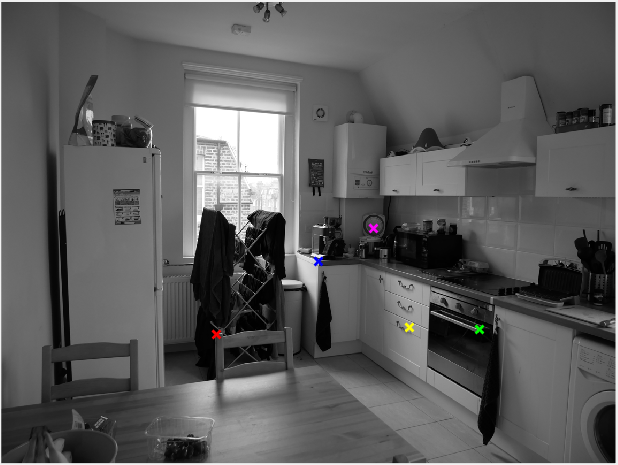
\includegraphics[width=\textwidth]{pic/manualA}
      \caption{Image A, original image}
      \label{fig:manualA}
    \end{subfigure}
    ~
    \begin{subfigure}{0.45\linewidth}
      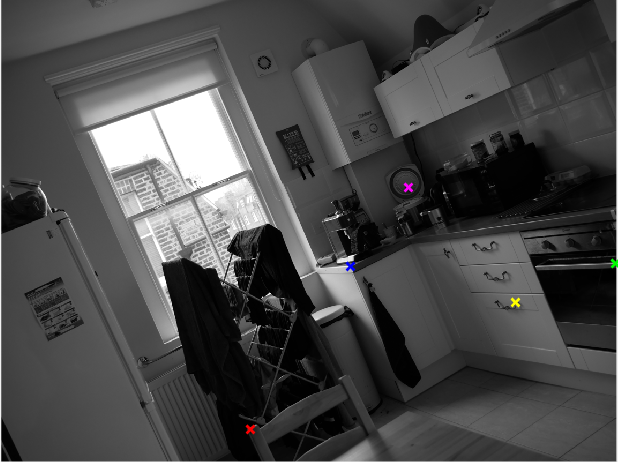
\includegraphics[width=\textwidth]{pic/manualB}
      \caption{Image B, zoomed by factor 1.5 and tilted by 20\degree}
      \label{fig:manualB}
    \end{subfigure}

	\caption{Example of manually selected data points on images}
  \label{fig:manual}
\end{figure}

\subsection{Automatic Feature Detection}

% Discuss need for interest point selection
For many computer vision applications, detecting features within an image or the same features within multiple images is crucial. These features can take a number of shapes, such as edges or corners. Once the same detector is run on two images with some of the same features, such as overlapping features in a panorama, the features can be automatically matches and a transformation estimated between the images.

% Discuss implemented selectors - TODO discuss the example images?
Both Hessian and Harris selectors have been implemented for this application. Both differentiate the given image twice and compare the results to a threshold, where calculations with the results vary depending on the detector. From subjective use of each detector, the Harris algorithm was found to perform more effectively. Both algorithms are based on code written by Svetlana Lazebnik \cite{harrisdetector}, and may be found in the Appendix as files \texttt{hessian.m} and \texttt{harris.m}. Images showing interest points detected by the two detectors are shown in Figure \ref{fig:detectors}. These images show an unexpected result in that many of the detected features seem to be part of uniform patches of image; this may suggest an insufficiently large threshold.

\begin{figure}[!ht]
  \captionsetup[subfigure]{position=b}
  \centering
    \begin{subfigure}{0.45\linewidth}
      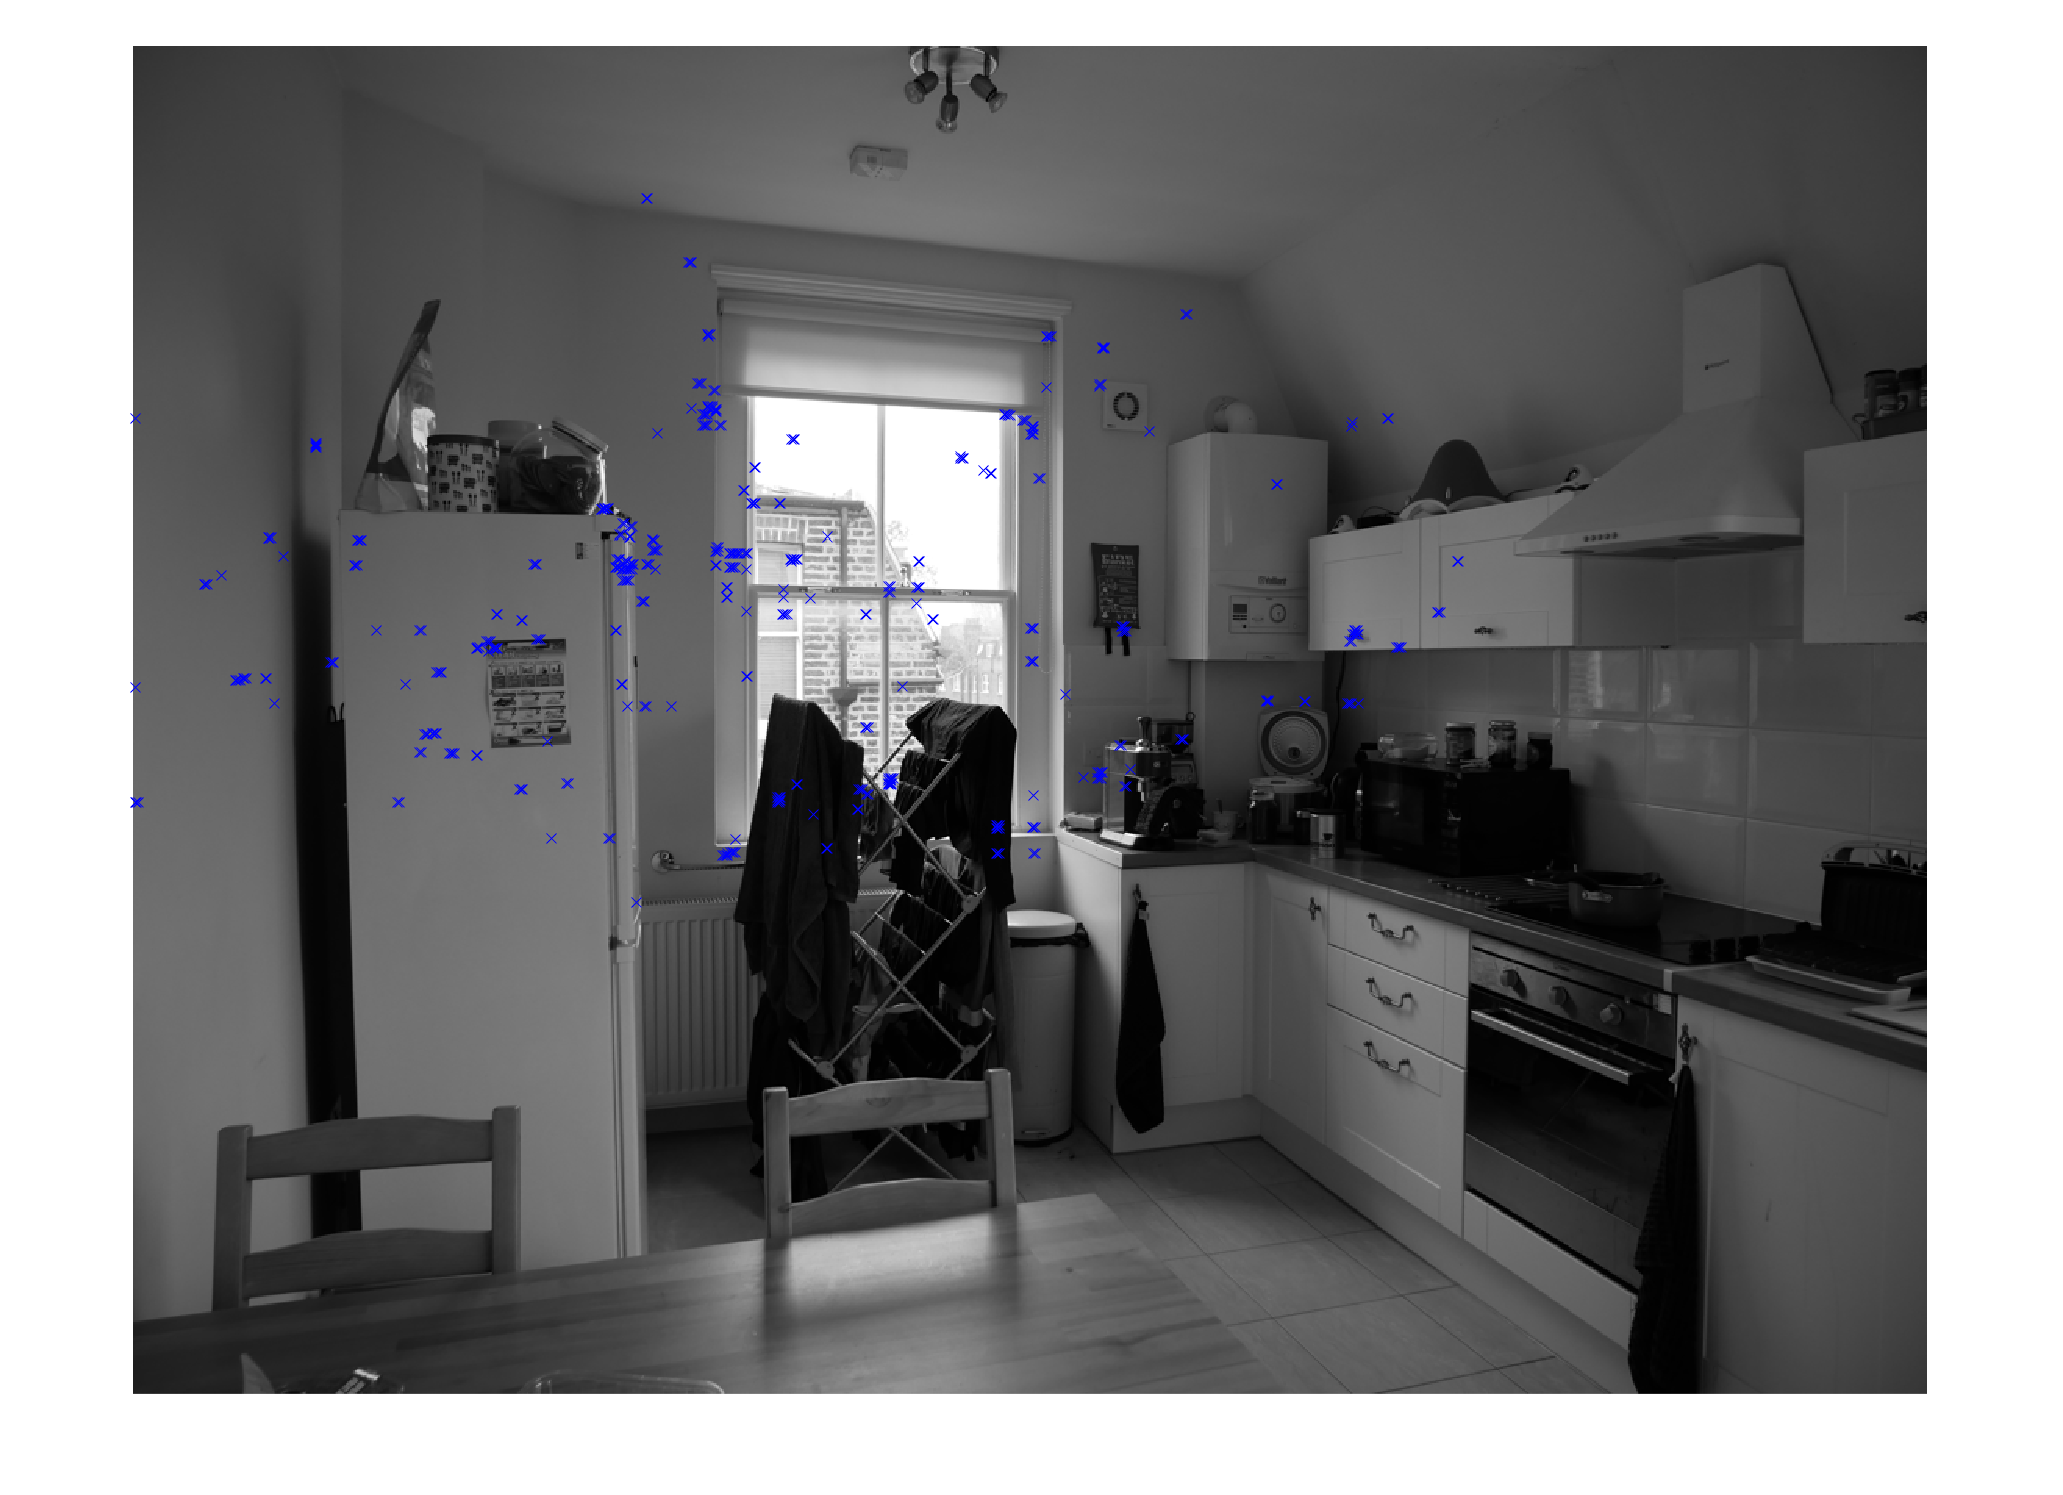
\includegraphics[width=\textwidth]{pic/hessian1e8}
      \caption{Image with Hessian detector, threshold $10^8$}
      \label{fig:hessian1e8}
    \end{subfigure}
    ~
    \begin{subfigure}{0.45\linewidth}
      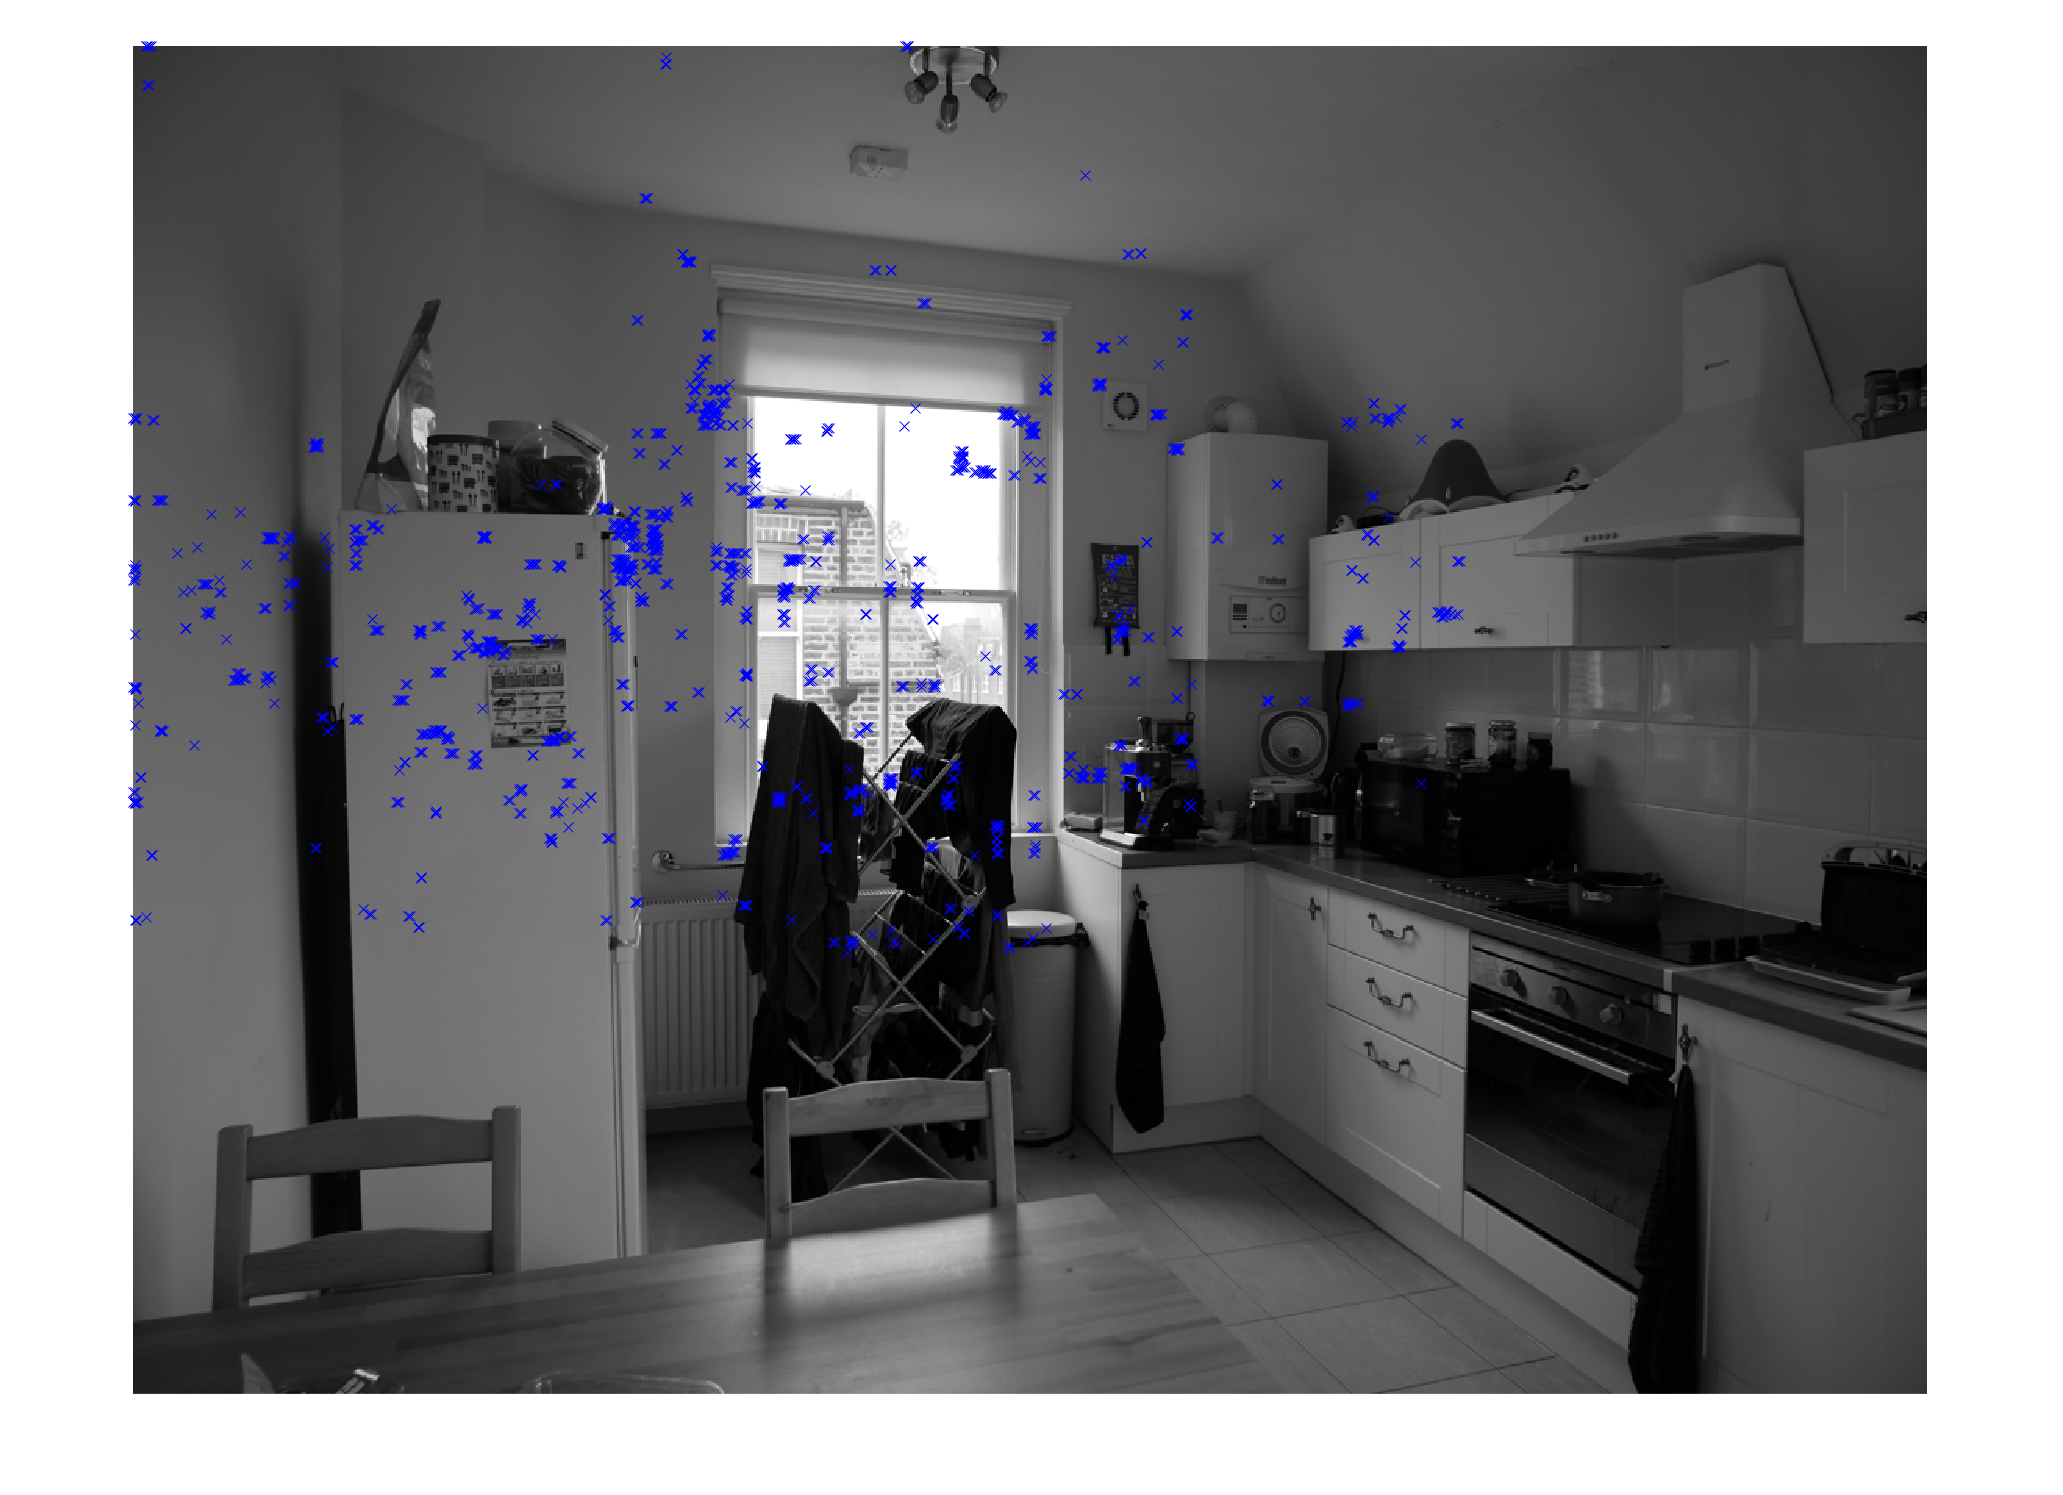
\includegraphics[width=\textwidth]{pic/harris3000}
      \caption{Image with Harris detector, threshold 3000}
      \label{fig:harris3000}
    \end{subfigure}

	\caption{Examples of Harris and Hessian detectors operating on Kitchen image}
  \label{fig:detectors}
\end{figure}

% Discuss need for description & our implementation
Once features have been detected in the image, these points must have some description to allow comparison with other points. At first, each interest point was used at the top left corner of a fixed-size patch, limiting the point so as not to cross the border. However, this removed some information due to the border limiting and the patch position missing out on rotation information if matching between images; therefore, the interest point is the centre of a patch in a padded image, and the descriptor of that patch is a simple histogram. The padded image is found by replicating the border pixels outwards. This may be found in the Appendix as \texttt{describe.m}.

% Discuss patch matching implementation - could really do with a side-by-side with lines connecting matched patches
Once each interest point has a corresponding descriptor, the points from two different images can be compared. The simplest method for comparing these descriptors is to use nearest neighbour (NN) matching, which interprets the difference in histograms as an error, and matches the points with the least error. Furthermore, the interest points from each image are considered in turn, and only if a pair of patches are both nearest neighbours to each other are they considered to match. The algorithm for this is shown in  the Appendix as \texttt{matchPatches.m}. 

An example image of two images with matching points is shown in Figure \ref{fig:matched}. The images used are the same as in Figure \ref{fig:manual}, but the threshold of 3000 with the Harris detector were used, which would indicate a similar number of feature points as in Figure \ref{fig:harris3000}. After NN matching, the number of points has been vastly reduced and mostly correspond, with a couple of exceptions, such as the green line between the coffee pot and the coffee machine pod. These points are not the same, but the surrounding area is very similar, which causes the error.

% I did also create this figure with showMatchedFeatures, but I found it really hard to spot where the differences are, so I did it like this. I can upload the matchedFeatures version if you want, just ask
\begin{figure}[!ht]
  \centering
  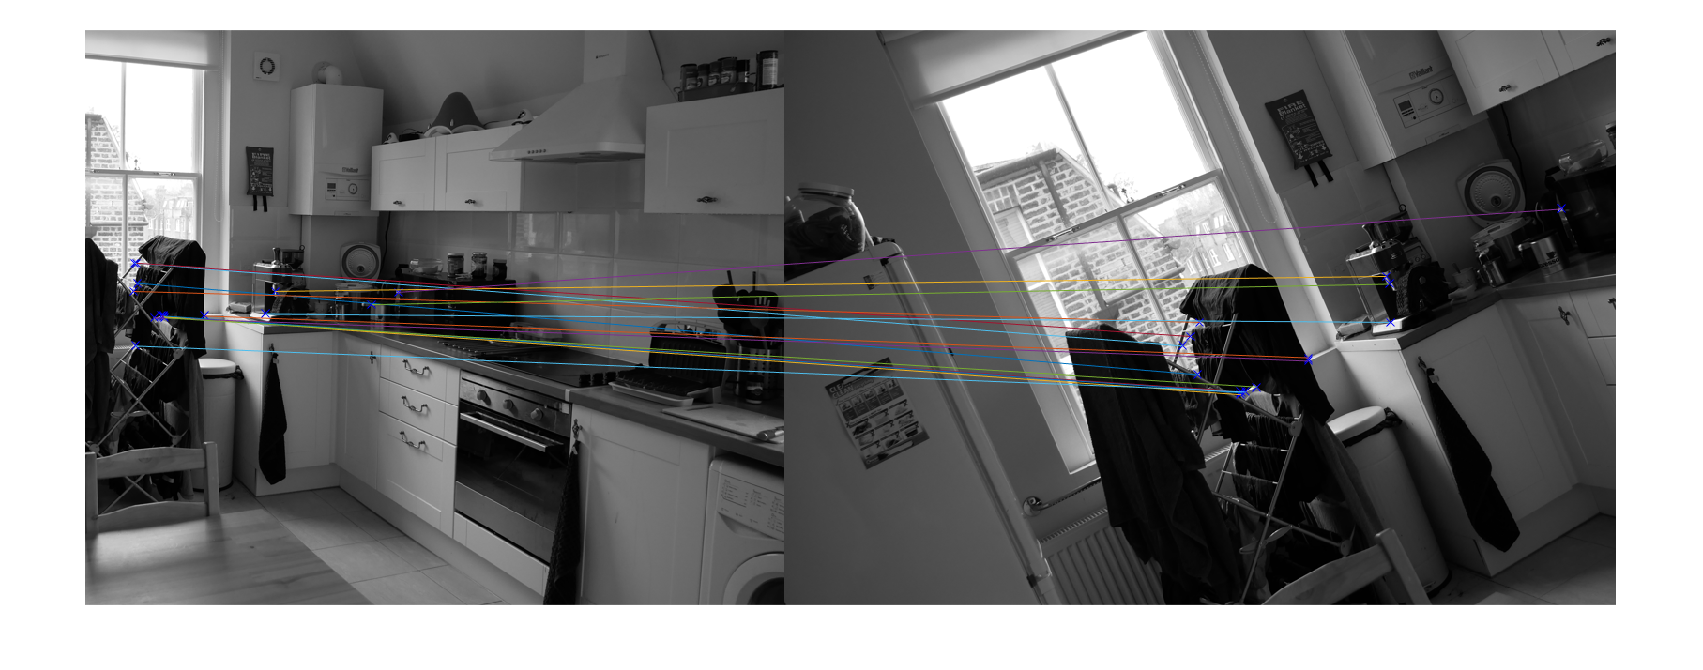
\includegraphics[width=\linewidth]{pic/matches}
  \caption{Matched patches between original image and image zoomed by factor 1.5 and tilted by 20\degree}
  \label{fig:matched}
\end{figure}


% \begin{enumerate}
%     \item Harris Detector Method. PIC: img1 with points on it, show with different thresholds.
%     \item Patch Extraction and Features Method. PIC: Example patches extracted, resulting histograms example. Do we definitely have to visualise this? Seems like it would take loads of space
%     \item NN Matching Method PIC: Using img1 and img2 with
%     \texttt{showMatchedFeatures(imgA, imgB, matchedPoints1, matchedPoints2);} to show result.
% \end{enumerate}

\subsection{Transformation Estimation}

% Need to discuss homography matrix estimation and show example

The matching pairs of points can be used to estimate the transformation matrix between the two images, known as the homography matrix. The homography matrix is \textbf{H}, and must satisfy Equation \ref{eqn:homography}, where \textbf{x} is the original point and $\textbf{x}'$ is the destination point after the transformation. The method for this is discussed in the course notes \cite{notes}; as such, examples of transformations will be shown, with the full details of implementation given in the source code in the Appendix, file \texttt{estTransformMat.m}.

\begin{equation} \label{eqn:homography}
\textbf{x}' = \textbf{Hx}
\end{equation}

An example of an estimated homography matrix is given in Equation \ref{eqn:homographyEstimated}, where the images used in Figure \ref{fig:manual} were again used to estimate a transformation. The result of transforming Image A to fit Image B is shown in Figure \ref{fig:homography}, which used manually selected user points as corresponding co-ordinates and estimated an accurate homography matrix. The matrix is considered accurate as the two images overlap to form grayscale in the centre. There is a slight error, shown by blurring around sharp edges where the green and purple do not match correctly.

\begin{equation} \label{eqn:homographyEstimated}
\textbf{H} = \begin{bmatrix}
    1.3964 & 0.5742 & -455.55 \\
    -0.5984 & 1.3651 & 190.96 \\
    0.0000 & -0.0000 & 1.0000
\end{bmatrix}
\end{equation}

\begin{figure}[!ht]
  \centering
  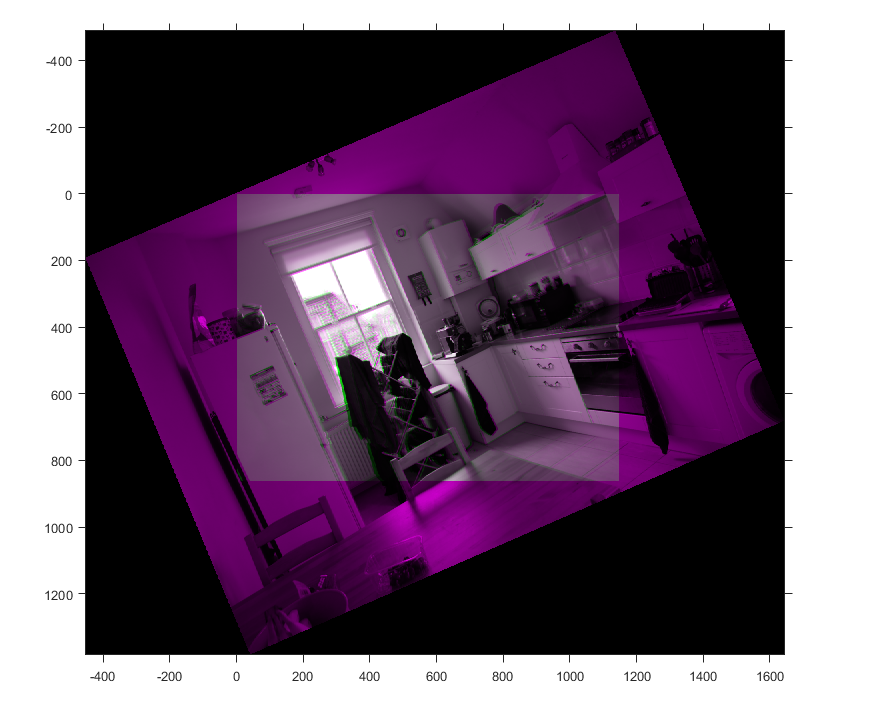
\includegraphics[width=\linewidth]{pic/homographyExample}
  \caption{Image A (purple) transformed and overlaid on Image B (green)}
  \label{fig:homography}
\end{figure}

% Discuss errorHA method
To estimate how well a homography matrix matches the two sets of points together, a metric called the Homography Accuracy (HA) is used. This HA is calculated by taking the corresponding sets of points and transforming one set to fit the other using the given homography matrix. The error between the predicted and actual points is interpreted as the distance; the mean distance is the HA. The HA for the example shown in \ref{fig:homography} is $HA=0.0536$.

% Need to discuss fundamental matrix estimation (and show example?)
Another matrix used in computer vision is the fundamental matrix, which can be estimated using a series of corresponding points. This matrix can be used to constrain the possible locations of points in a second image from points in the first image given the fundamental matrix between the two images. The method itself is very similar to the homography matrix, except that the relation in Equation \ref{eqn:fundamental} is used instead of that in Equation \ref{eqn:homography}. The code for implementation is given in the Appendix as file \texttt{estFundamentalMat.m}.

\begin{equation} \label{eqn:fundamental}
\textbf{x}'^T\textbf{Fx} = 0
\end{equation}

% Discuss epipole lines and show example
% TODO actually sort out epipole lines

The fundamental matrix can be used to constrain the search space from points in one image to the same scene points in the second image by giving the equation of a line $\textbf{l}=\textbf{Fx}$, such that the correct point on the line \textbf{l} satisfies Equation \ref{eqn:fundamental}. This is known as the epipole line. The same manual data and images used for Figure \ref{fig:homography} are used to estimate a fundamental matrix, given in Equation \ref{eqn:fundamentalEstimated}. This matrix \textbf{F} is then used to generate epipolar lines, shown in Figure TODO.

\begin{equation} \label{eqn:fundamentalEstimated}
\textbf{F} = \begin{bmatrix}
     0.0000 & -0.0001 &  0.0017 \\
     0.0001 &  0.0000 & -0.0355 \\
    -0.0191 &  0.0280 &  1.0000
\end{bmatrix}
\end{equation}

% TODO show epipole lines image

% \begin{enumerate}
%     \item Homography Matrix Estimation Method PIC: img1 with img2
%     \item Fundamental Matrix Estimation Method
%     \item ErrorHA Method (also does projecting)
%     \item Needs to be done lol. ``Implement a method for calculating epipolar line given point coordinates and a
% Fundamental matrix between two images. Display that line on an image in Matlab.''
% \end{enumerate}

\section{Question - Image Geometry}
\subsection{Homography with HG Pictures}
\subsubsection{Reduced Size}
0.5995 Error
\subsubsection{Manual vs. Automatic}
Harris 4K points for 500 threshold
\subsubsection{Number of Correspondences}

\subsection{Stereo Vision With FD Pictures}


\cite{notes}


%-------------------------------------------------------------------------------
% Conclusion
%-------------------------------------------------------------------------------
\section{Conclusion}
Lorem ipsum dolor sit amet, consectetur adipiscing elit. Phasellus gravida viverra sollicitudin. Nulla ornare enim in ante auctor rhoncus a vel nulla. Nulla condimentum massa rhoncus, sodales arcu a, euismod nulla. Proin viverra mauris at massa molestie, a ultricies tortor fermentum. Duis consectetur, ante a tincidunt euismod, augue diam varius dolor, ut vestibulum orci est sit amet mi. Aenean sit amet metus vitae sem malesuada tempus. Vivamus placerat ornare erat quis tincidunt. In quis massa aliquet, pellentesque magna vitae, luctus eros.

%-------------------------------------------------------------------------------
% References
%-------------------------------------------------------------------------------
\bibliographystyle{unsrt}
\bibliography{mlcv_refs}

%-------------------------------------------------------------------------------
% Appendix(ces)
%-------------------------------------------------------------------------------
\onecolumn
\section*{Appendix}

\subsection*{q1\_manual.m}
\lstinputlisting[style=Matlab-editor]{src/q1_manual.m}
\newpage

\subsection*{hessian.m}
\lstinputlisting[style=Matlab-editor]{src/hessian.m}
\newpage

\subsection*{harris.m}
\lstinputlisting[style=Matlab-editor]{src/harris.m}
\newpage

\subsection*{describe.m}
\lstinputlisting[style=Matlab-editor]{src/describe2.m}
\newpage

\subsection*{estTransformMat.m}
\lstinputlisting[style=Matlab-editor]{src/estTransformMat.m}
\newpage

\end{document}
